%%%%% Description: history of (weak) consistency models in the context of distributed systems. %%%%%
%%%%% Date: July 14, 2016 %%%%%
%%%%% Author: Hengfeng Wei %%%%

\documentclass{standalone}

\usepackage{tikz}
\usetikzlibrary{positioning, shapes, shapes.symbols, backgrounds, fit, arrows.meta, calc}

\begin{document}
\begin{tikzpicture}[comment/.style = {align = center}]
  %%%%%%%%%% Begin: years and papers %%%%%%%%%% 
  % \x: x coordinate; \y: year; \n: name; \lbl: label
  \foreach \x/\y/\n/\lbl in {
  	1/$1995$/eventual/eventual consistency, 
	6/$2000$/cap/CAP theorem, 
	11/$2006$/bigtable/Bigtable@Google, 
    14/$2007$/amazon/Dynamo@Amazon, 
    18/$2012$/pacelc/PACELC tradeoff} {
	\node[star, star points = 5, minimum size = 3pt, draw = red, fill = yellow, line width = 2pt] (\x) at (\x, 5) {};
	\node[below = 0.50cm of \x] (\y) {\y};
	\node[above = 0.50cm of \x, align = center] (\n) {\lbl};
  }

  \path[draw = red, dashed, very thick] (1) to (6) to (11) to (14) to (18);
  %%%%%%%%%% End: decades and systems %%%%%%%%%% 

  %%%%% cap theorem %%%%%
  \node[above = of cap] (cap-fig) {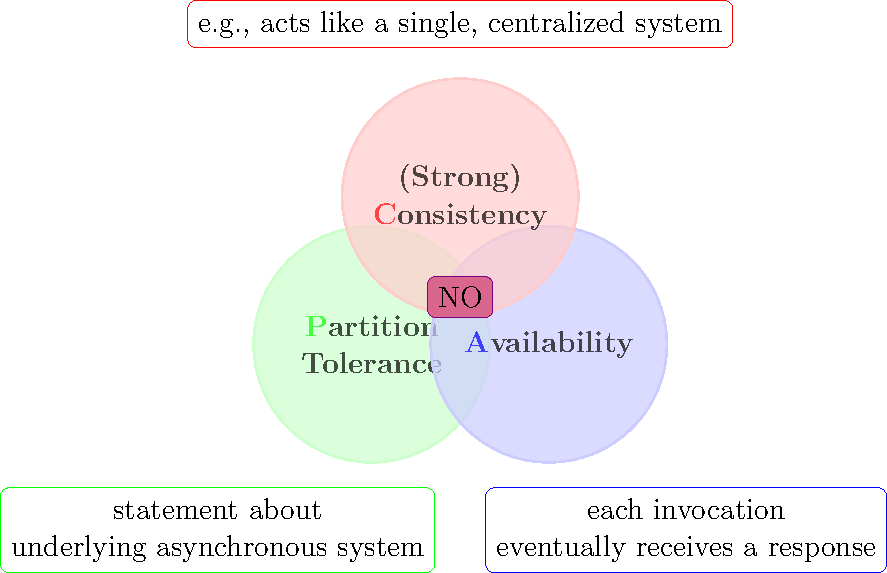
\includegraphics[scale = 0.40]{figs/cap-theorem.pdf}}; 
\end{tikzpicture}
\end{document}
